\chapter{Applications to Neuromorphic Hardware}
\label{chapt:results}

\section{Learning on SpiNNaker}
\label{sec:learn-spinnaker}

This section is taken from \citep{knight2016}.

The biological brain is a highly plastic system within which the efficacy and structure of synaptic connections are constantly changing in response to internal and external stimuli.
While numerous models of this plastic behavior exist at various levels of abstraction, how these mechanisms allow the brain to learn meaningful values is unclear.
The Neural Engineering Framework~(NEF) is a hypothesis about how large-scale neural systems represent values using populations of spiking neurons, and transform them using functions implemented by the synaptic weights between populations.
By exploiting the fact that these connection weight matrices are factorable, we have recently shown that static NEF models can be simulated very efficiently using the SpiNNaker neuromorphic architecture.
In this paper, we demonstrate how this approach can be extended to efficiently support both supervised and unsupervised learning rules designed to operate on these factored matrices.
We then present a heteroassociative memory architecture built using these learning rules and prove that it is capable of learning a human-scale semantic network.
Finally we demonstrate a \numprint{100000} neuron version of this architecture running on the SpiNNaker simulator with a speed-up exceeding 150x when compared to the Nengo reference simulator.

\begin{figure}
  \centering
  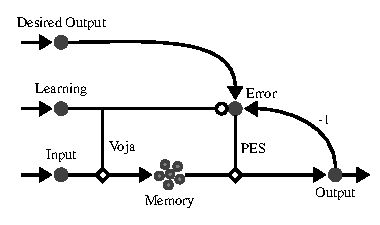
\includegraphics{voja-associative-network}
  \caption{Heteroassociative memory network using both PES and Voja learning rules.}
  \label{fig:voja-associative-network}
\end{figure}

We now proceed by applying both supervised and unsupervised learning to a single population in order to construct a network that can learn associations between pairs of vectors online.
This {\it heteroassociative memory} network is akin to a distributed hash table, in which distinct input vectors are associated with arbitrary output vectors.
The NEF has already been used to build a static memory that can recall \numprint{117659} associations between pairs of 512-dimensional vectors, using over \numprint{2500000} spiking neurons in a single layer~\citep{crawford2015}.
This model was used to traverse the relations in WordNet, a human-scale semantic network.
The output vectors can also be learned online by using the supervised PES rule to minimize the error between the output of the memory and the desired vector.
However supervised learning on its own is inadequate if we lack prior knowledge of the possible inputs to the network. If two distinct inputs cause the same neuron to fire then their two output vectors will depend on one another.
% By "inadequate", we mean that in theory one can still do it without Voja, but there is a lot of wasted space when setting the intercepts to prevent all overlap (not the same as setting the intercepts to prevent collisions), and the firing rates will be too low for most neurons. So it does not scale (unpublished?).
In the case when we cannot assume nearby inputs are associated with similar outputs we require a sparse encoding of the input vectors such that any given neuron will fire in response to at most one distinct input.
Sparse coding has been commonly observed in the hippocampus, where as few as 50 to 200 cells may participate in the encoding of a single representation \citep{Quiroga2012, Mainetti2015}.
This kind of sparsity may be achieved by using the unsupervised Voja rule to tune the encoders of the memory towards its inputs~\citep{voelker2014a} as shown in \figurename~\ref{fig:plasticity_nef/voja_encoders}.
%However, when using a traditional hardware architecture, we cannot expect to learn over 100,000 associations within a single simulation in any reasonable length of time.
%We also need lower dimensionality to run on SpiNNaker

To construct this network, we let $M$, $D$, and $K$ correspond to the number of associations, dimensionality, and the number of neurons per association, respectively.
We initialize the encoders of all $N = M \times K$ neurons using the {\it Sobol sequence} to generate a low-discrepancy set of points on the $(D-1)$-cube~\citep{Sobol1967}, and then use the inverse distribution and spherical coordinate transformation derived by \citet{fang1994} to map this sequence onto the uniform $D$-sphere.

We set $\alpha_i$ and $\beta_i$ from (\ref{eq:encoding}) such that the maximum firing rate of each neuron is $r_i$ (achieved when the input is equal to the encoder) and firing occurs with probability $\frac{1}{M}$.
This is accomplished by solving the system of equations,

\begin{align}
  \alpha_i c + \beta_i &= J_i^{0} \label{eq:firing-min} \\
  \alpha_i + \beta_i &= J_i^{max} \label{eq:firing-max} \\
  1 - F_D(c) &= \frac{1}{M} ,     \label{eq:intercept} % c &= F_D^{-1}(1 - \frac{1}{M})
\end{align}
%
where $J_i^0$ is the smallest constant input current to $G_i \left[ \cdot \right]$ that results in firing, $J_i^{max}$ is the current that produces a firing rate of $r_i$, and $F_D$ is given by the cumulative distribution:
%
\begin{equation}
  \label{eq:cosine}
  F_D(c) \propto \int_{-1}^c (1 - y^2)^{\frac{D - 3}{2}} \, dy, \quad |c| \le 1 .
\end{equation}
%
This distribution corresponds to the dot product of any unit vector with a uniformly chosen $D$-dimensional encoder.
By (\ref{eq:firing-min}), the $i^\mathrm{th}$ neuron will fire in response to a unit input $\V{x}$ if and only if $\V{e}_i \cdot \V{x} \ge c$.
Therefore, (\ref{eq:intercept}) guarantees that $N / M = K$ neurons are expected to fire in response to any unit vector.

The chosen value of $c$ also determines the maximum allowable similarity between two input vectors.
For any two distinct input vectors $\V{x}_i$ and $\V{x}_j$, we require $\V{x}_i \cdot \V{x}_j < c$ for all $i \ne j$.
Otherwise, an encoder that converges to $\V{x}_i$ with Voja will still fire in response to the input $\V{x}_j$, and vice-versa.
Whenever this occurs, the current association will overwrite the previously learned value.
The task of enforcing a maximum similarity is connected to the {\it kissing problem}~\citep{Conway1999}.
The {\it Leech lattice} gives us an optimal solution that is straightforward to compute for $D=24$.
In particular, we choose our input vectors from the set of points in the lattice closest to the origin, normalized to unit length. 
There are \numprint{196560} such points on the 24-sphere, each separated by an angle of $\theta \ge \frac{\pi}{3}$.
These points are also closely related to the codewords of the linear error-correcting {\it Golay code}.
The possible input vectors may be interpreted as spherical codewords that are optimally distant from one another in Euclidean space.
This has the benefit of producing a distinct set of neural responses that are robust to the magnitude of $\|\V{x} - \V{\hat{x}}\|$, which is precisely the approximation error minimized by (\ref{eq:rmse}).
As $\V{x}_i \cdot \V{x}_j \le cos(\theta) \|\V{x}_i\| \|\V{x}_j\| = 0.5$, we require $c > 0.5$ in order to prevent collisions.
This occurs if and only if $M > (1 - F_{24}(0.5))^{-1}$ by (\ref{eq:intercept}).
Thus, we may efficiently pack a large number of associations ($\numprint{184} \le M \le \numprint{196560}$) into a $24$-dimensional space, and then use Voja to tune each neuron to fire maximally in response to at most one input.

In order to compare our SpiNNaker implementation of the PES and Voja learning rules to the reference NEF implementation~(Nengo~\citep{bekolay2014}), we simulated the heteroassociative memory network described in \S\ref{sec:memory} at scales ranging from $M=250$ to $M=2000$ on both a 48-chip SpiNNaker machine and a standard desktop PC (3GHz AMD Athlon II X3 445).

For our benchmark, we present $M$ pairs of $24$-dimensional input and output vectors to the memory, each for \SI{200}{\milli\second} during a training phase, with learning rates of $\kappa = 0.01$ and $\eta = 0.005$ for PES and Voja, respectively.
%The simulated neuron model $G_i \left[ \cdot \right]$ was chosen to be the {\it leaky integrate-and-fire} neuron with a capacitance of $\tau_{rc} = \SI{20}{\milli\second}$ and a refractory period of $\tau_{ref} = 2$\,ms.
We then tested recall by disabling learning and presenting the same sequence of input vectors to the population of neurons, each for \SI{50}{\milli\second}.

The accuracy of the system was evaluated by comparing the value at the output node of the network during recall with the output vector presented during training.
Both the SpiNNaker and reference simulator correctly recalled the output vectors with a consistent RMSE of approximately \num{0.2} at all scales.
However as Table~\ref{tab:results/memory_scale} shows, while the SpiNNaker simulations ran in real-time (\SI{0.25}{\second} per association), the time taken by the Nengo reference simulator grew quadratically -- over $150\times$ slower than real-time in the largest configuration.

\begin{table}
  \centering
  \caption{Simulation times on SpiNNaker and Nengo reference simulator}
  \label{tab:results/memory_scale}
\sisetup{table-number-alignment=right, table-figures-decimal=0}
\begin{tabular}{S S S r r}
  \toprule
  \multicolumn{2}{c}{Number of} & \multicolumn{2}{c}{Simulation time / minutes} \\
  {Associations} & {Neurons} & {SpiNNaker} & {Nengo Reference}\\
  \midrule
    250 & 12500 & 1.0 & 20.1 \\
    500 & 25000 & 2.1 & 75.5 \\
    1000 & 50000 & 4.2 & 309.0 \\
    2000 & 100000 & 8.3 & 1307.1 \\
  \bottomrule
\end{tabular}
\end{table}

The large number of afferent synapses associated with each neuron make simulating synaptic plasticity on SpiNNaker very computationally expensive.
In this paper we built on our previous work~\citep{mundy2015} to show that, by taking advantage of the factorable synaptic weight matrices used by the NEF and not simulating individual synapses, we can simulate both plastic and static spiking neural networks highly efficiently.
To demonstrate the benefits of this approach we implemented two biologically plausible learning rules on SpiNNaker and, using these, built a heteroassociative memory network that we proved to be capable of storing a human-scale semantic network.
By simulating this memory network at scales of up to \numprint{100000} neurons, we demonstrated that these two learning rules only reduce the number of neurons each SpiNNaker core can simulate by \SI{6}{\percent} and that by using SpiNNaker rather than a standard desktop PC, simulation times are reduced by over $150\times$.

\section{Dynamical Systems Benchmarks}

Compare Braindrop versus Loihi
\TODO{Running on Eric's integrator-accuracy branch}

\subsection{Integrator}
\label{sec:integrator}

\begin{figure}
  \centering
  \begin{subfigure}{.5\textwidth}
    \centering
    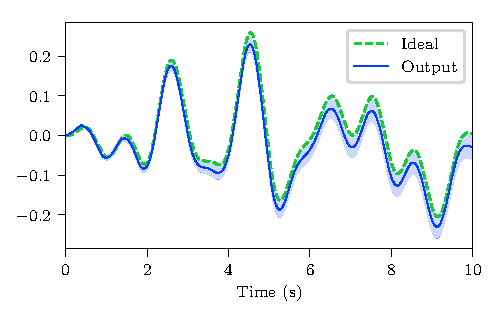
\includegraphics[width=\linewidth]{braindrop-integrator}
    \caption{Braindrop Chip}
    \label{fig:dn-braindrop}
  \end{subfigure}%
  \begin{subfigure}{.5\textwidth}
    \centering
    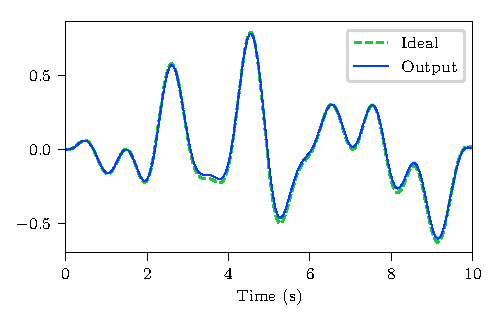
\includegraphics[width=\linewidth]{loihi-integrator}
    \caption{Loihi Emulator}
    \label{fig:dn-loihi}
  \end{subfigure}
  \caption{ \label{fig:integrator-neuromorphic}
    An integrator running on state-of-the-art neuromorphic hardware.
    The ideal solution is plotted against the mean's 95\% confidence interval, bootstrapped from $200$ trial simulations.
    (a)~Braindrop implementation, reproduced from \citet[][Figure~15]{braindrop2019}, using \numprint{1024} neurons. 
    (b)~Loihi Emulator (v0.4.0) implementation, using \numprint{256} neurons.
    See text for details.
  }
\end{figure}

The integrator, $\theta \dot{\V{x}}(t) = \V{u}(t)$, is a dynamical system used extensively by Spaun~\citep{eliasmith2012} and many other NEF and SPA models~\citep[][to name a few]{singh2004, trujillo2014a, rasmussen2017} for cognitive tasks involving working memory.
This system can persist information about the history of an input signal, starting from $t_0$ and extended indefinitely throughout time, as characterized by its solution:
$$\V{x}(t) = \V{x}(t_0) + \frac{1}{\theta} \int_{t'=t_0}^{t} \V{u}(t')\, dt' \text{.}$$
The parameter $\theta$ is a time-constant that controls how quickly the memory integrates new information.\footnote{
This parameter is useful for dimensional analysis, and when considering the transfer function, $\frac{\V{X}(s)}{\V{U}(s)} = \left( \theta s \right)^{-1}$.}
For example, beginning from an initial state of $\V{x}(t_0) = \V{0}$, if we hold the input constant at $\V{u}(t) = \V{v}$ for $\theta$ seconds ($t_0 < t \le t_0 + \theta$), and then clamp the input to $\V{u}(t) = \V{0}$ thereafter ($t > t_0 + \theta$), then $\V{x}(t) = \V{v}$ will ``store'' the vector $\V{v}$ indefinitely.
More generally, any finite set of nonlinear differential equations can be described as the integration of an input vector that is some nonlinear function of the state-vector---augmented to also include $\V{u}(t)$---as in $\theta \dot{\V{x}}(t) = \V{f}\left({\V{x}(t)}\right)$.
The nonlinearity $\V{f}(\cdot)$ may then be supported by a pool of neurons encoding the state-vector, as explained in section~\ref{sec:nef}.
Thus, the integrator is a basic component that can be used to implement more complicated nonlinear dynamical transformations, such as those involved in adaptive motor control~\citep{dewolf2016}.
We therefore use the integrator, implemented by a pool of spiking neurons using the methods of the NEF, as a benchmark for evaluating the ability of neuromorphic hardware to implement nonlinear dynamical systems.

In Figure~\ref{fig:integrator-neuromorphic}, we instantiate a one-dimensional integrator ($\theta = 1$\,s) on both Braindrop (1024 neurons) and Loihi (256 neurons).\footnote{
We use four times fewer neurons on Loihi versus Braindrop, as increasing the pool size leads to a bug in the \texttt{nengo-loihi}~v0.4.0 software.}
In both cases, the input signal is a white-noise test signal, band-limited to $1$\,Hz.
Both the ideal and the spiking activity are filtered with a lowpass ($\tau = 200$\,ms).
On Braindrop (see Figure~\ref{fig:integrator-neuromorphic}~(a), reproduced from \citet[][Figure~15]{braindrop2019}), we compensate for the distribution of synaptic time-constants, arising from transistor mismatch in the analog circuitry, using the methods of \citet{voelker2017iscas} and section~\ref{sec:mismatch}.
The chip is configured to maximize the synaptic time-constants; the empirically measured mean is $179.3$\,ms, with a standard deviation of $53.8$\,ms.
On Loihi (see Figure~\ref{fig:integrator-neuromorphic}~(b)), we set $\tau = 200$\,ms, and use the methods of \ref{sec:linear-extensions} to discretize the integrator according to the simulation time-step ($dt = 1$\,ms).

\TODO{Also used ReLU for Loihi, and some hacking of the spike-generator.}

In either case, the 95\% confidence intervals include the ideal across nearly the entire $10$\,s simulation.
This implies that the sum of any error, whether related to spiking, representation, or otherwise, has a mean value of approximately zero.
We remark that Loihi gives much more consistent trial-to-trial results, due to the all-digital nature of the chip, and lack of temperature-induced variability.
Advanced methods that can be used to provide temperature-invariant decodes in Braindrop have been recently developed by \citet{reidpint2019}, although they require external measurements of the device's temperature, and thus were not employed by this experiment.

\subsection{Delay Network}

\begin{figure}
  \centering
  \begin{subfigure}{.5\textwidth}
    \centering
    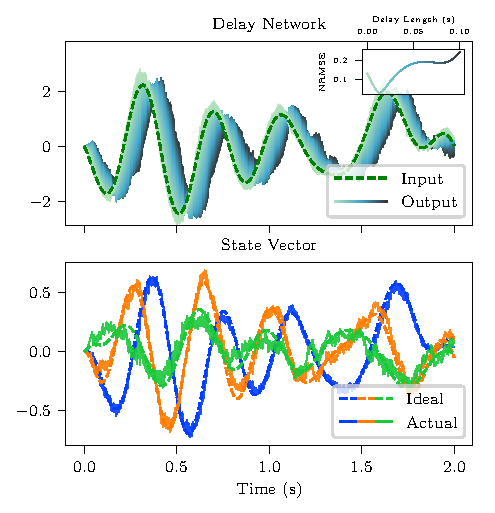
\includegraphics[width=\linewidth]{dn-braindrop}
    \caption{Braindrop Chip}
    \label{fig:dn-braindrop}
  \end{subfigure}%
  \begin{subfigure}{.5\textwidth}
    \centering
    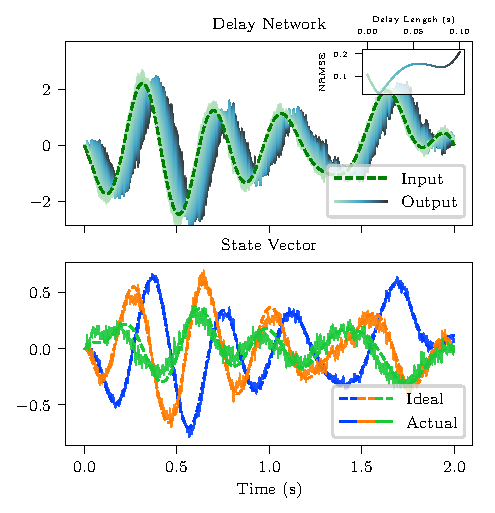
\includegraphics[width=\linewidth]{dn-loihi}
    \caption{Loihi Emulator}
    \label{fig:dn-loihi}
  \end{subfigure}
  \begin{subfigure}{\textwidth}
    \centering
    \vspace{2em}
    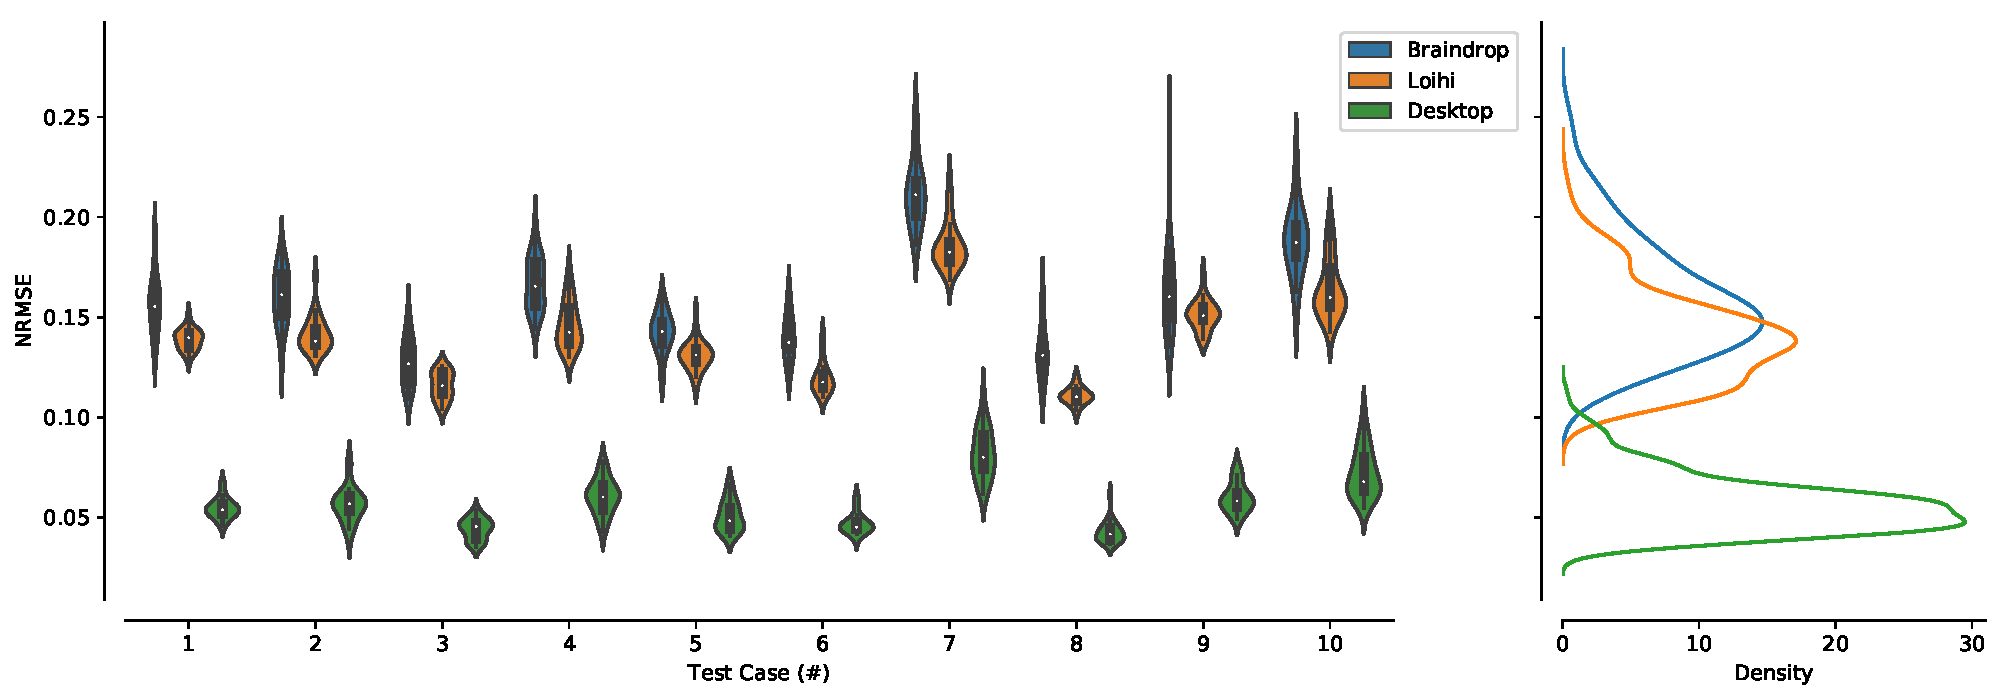
\includegraphics[width=\linewidth]{dn-trials}
    \caption{Overall Error}
    \label{fig:dn-trials}
  \end{subfigure}
  \caption{ \label{fig:dn-neuromorphic}
    Delay Network~(DN; $q=3$, $\theta=100$\,ms; chapter~\ref{chapt:delays}) running on state-of-the-art neuromorphic hardware.
    (a)~Braindrop implementation, reproduced from \citet[][Figure~16]{braindrop2019}. 
    (b)~Loihi Emulator (v0.4.0) implementation.
    (c)~Overall error~(NRMSE) for Braindrop, Loihi, and a standard desktop CPU, across 10 test cases, with 25 randomly initialized network configurations per test case.
    The simulations shown in (a) and (b) correspond to a randomly chosen trial from the first test case in (c).
    See text for details.
  }
\end{figure}


We now instantiate the same Delay Network~(DN) from chapter~\ref{chapt:delays} on state-of-the-art neuromorphic hardware (see Figure~\ref{fig:dn-neuromorphic}).
This system may be conceptualized as an entirely different kind of memory that persists not the sum of the input signal, but finite windows of input history.
In other words, the DN ``buffers'' a sliding window of the input, which enables the computation of arbitrary nonlinear transformations across the window.
This can be used as a basic building block for working memory models that must represent not only \emph{what} has occurred, but also \emph{when} it has occurred in relation to everything else.

To implement the DN, three pools, each containing $128$ spiking neurons, are recurrently coupled to each other (and to themselves), and trained to optimally buffer a white-noise test signal---band-limited to $3$\,Hz---across a $100$\,ms sliding time-window.
Output spikes are filtered using a lowpass synapse with $\tau = 20$\,ms, and weighted to decode both the state-vector and the window of history.
On Braindrop~(see Figure~\ref{fig:dn-neuromorphic}~(a), reproduced from \citet[][Figure~16]{braindrop2019}), the chip is configured to use the default distribution of synaptic time-constants (mean $\tau \approx 18$\,ms).
\TODO{Grab and plot the distribution from the calibration data using the mapped xy coordinates for the 3 ensembles.}
On Loihi~(see Figure~\ref{fig:dn-neuromorphic}~(b)), performance is maximized by using all-to-all weight matrices, and setting the recurrent time-constant to $\tau=10$\,ms.
We also compare this to the reference Nengo simulator ($\tau=10$\,ms) running on a conventional desktop CPU to obtain a baseline level of performance.
The overall error, reported as bootstrapped 95\% confidence intervals across $10 \times 25$~trials, is
[0.156,~0.163] for Braindrop,
[0.146, 0.153] for Loihi (compared to [0.145, 0.151] for the emulator), and
[0.055,~0.059] for the CPU (see Figure~\ref{fig:dn-neuromorphic}~(c)).
